\documentclass{beamer}
\usepackage{amsmath}
\usepackage[english]{babel}
\usepackage{bbm}
\usepackage{graphicx}
\usepackage[utf8]{inputenc}
\usepackage{tikz}
\usepackage{wrapfig}

\usetikzlibrary{shapes,arrows}
\tikzstyle{block} = [rectangle, draw,% fill=blue!20, 
    text width=10em, text centered, rounded corners]%, minimum height=4em]
\tikzstyle{line} = [draw, -latex']

\mode<presentation>
\usetheme{Warsaw}

\DeclareMathOperator{\Tr}{Tr}

\bibliographystyle{unsrt}
\setbeamertemplate{caption}[numbered]

%\graphicspath{ {../images/} }

\title{Quantum nonlinear oscillator}
      
\author{Evgeny Anikin}
\institute{Skolkovo institute of science and technology}
\date{}

\begin{document}

\begin{frame}
    \titlepage
\end{frame}

\begin{frame}
    \frametitle{Problem Hamiltonian}
    \begin{equation}
       \hat{H} = \omega_0 a^\dagger a + \frac{\beta}{2} a^\dagger a^\dagger a a + 
                    E^*e^{i\Omega t} a + Ee^{-i\Omega t} a^\dagger 
    \end{equation}
    After substitution $\Psi = e^{i\Omega t a^\dagger a} \widetilde{\Psi}$ the Schroedinger equation 
    becomes
    \begin{equation}
        i\partial_t \widetilde{\Psi} = \hat{H}_{\mathrm{eff}}\widetilde{\Psi},
    \end{equation}
    with the effective Hamiltonian
    \begin{equation}
        \hat{H}_{\mathrm{eff}} = (\omega_0 - \Omega) a^\dagger a + 
                            \frac{\beta}{2} a^\dagger a^\dagger a a + 
                    E^* a + Ea^\dagger 
    \end{equation}
\end{frame}

\begin{frame}
    \frametitle{Classical description}
    \begin{columns}
        \begin{column}{0.5\textwidth}
            The quantum Heisenberg equation 
            \begin{equation*}
                i\frac{\partial\hat{a}}{\partial t} = -|\Delta|\hat{a} + 
                                \beta \hat{a}^\dagger \hat{a} \hat{a} + E
            \end{equation*}
            becomes
            \begin{equation*}
                i\frac{\partial a}{\partial t} = -|\Delta|a + \beta |a|^2 a + E
            \end{equation*}
            Classical energy:
            \begin{equation*}
                H = -\Delta |a|^2 + \frac{\beta}{2}|a|^4 + E^*a + Ea^*
            \end{equation*}
        \end{column}
        \begin{column}{0.5\textwidth}
            \begin{figure}[h]
                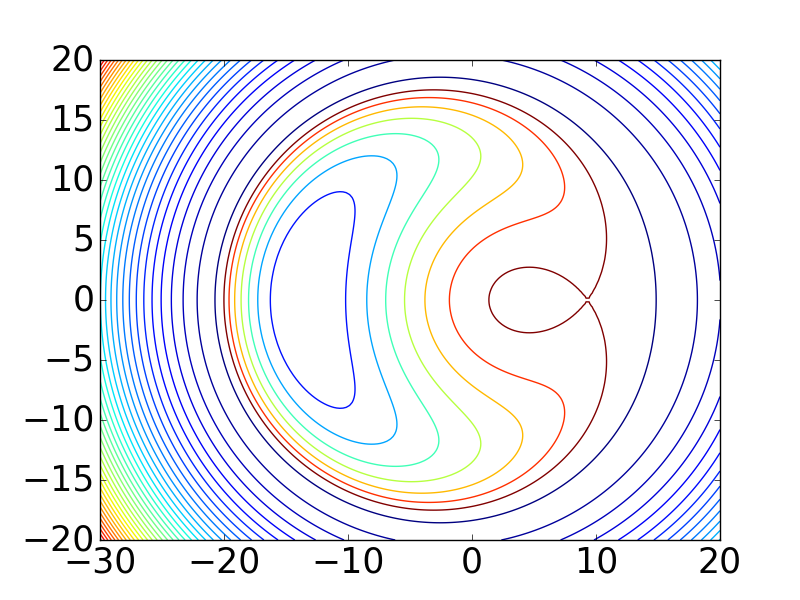
\includegraphics[width=0.9\textwidth]{classical_phase_portrait.png}
                \caption{Phase portrait of the classical nonlinear oscillator 
                         in the complex $a$ plane. $\Delta = -1$, $\beta = 1/12^2$, 
                        $E = 0.8 \sqrt{\frac{4\Delta^3}{27\beta}} = 3.70$ }
            \end{figure}
        \end{column}
    \end{columns}
\end{frame}

\begin{frame}
    \frametitle{Quantum description}
    Eigenvectors of the Hamiltonian have the form
    \begin{equation*}
        |\psi_n\rangle = \sum c_k |k\rangle
    \end{equation*}
    With any vector, it is possible to construct the quantity 
    $e^{-\frac{\bar{\xi} \xi}{2}}\langle \xi | \psi \rangle$, where $|\xi \rangle$ is a coherent 
    state. 
\end{frame}

\begin{frame}
    \frametitle{Reminder on coherent states}
    By definition, 
    $ \hat{a}|\xi \rangle = \xi|\xi \rangle $.
    That leads to a decomposition
    \begin{equation*}
        |\xi \rangle = e^{\xi \hat{a}^\dagger}|0\rangle = \sum \frac{\xi^n}{\sqrt{n!}} |n\rangle
    \end{equation*}
    An enormously important relation:
    \begin{equation*}
        \int d\bar{\xi} d\xi\, e^{-\bar{\xi}\xi} |\xi\rangle\langle\xi | = \mathbbm{1}
    \end{equation*}
    As a consequance, any state can be represented as an integral over coherent states.     
    
\end{frame}

\begin{frame}
    \frametitle{Eigenstates of the quantum Hamiltonian}
    \only<1>{\begin{figure}[h]
        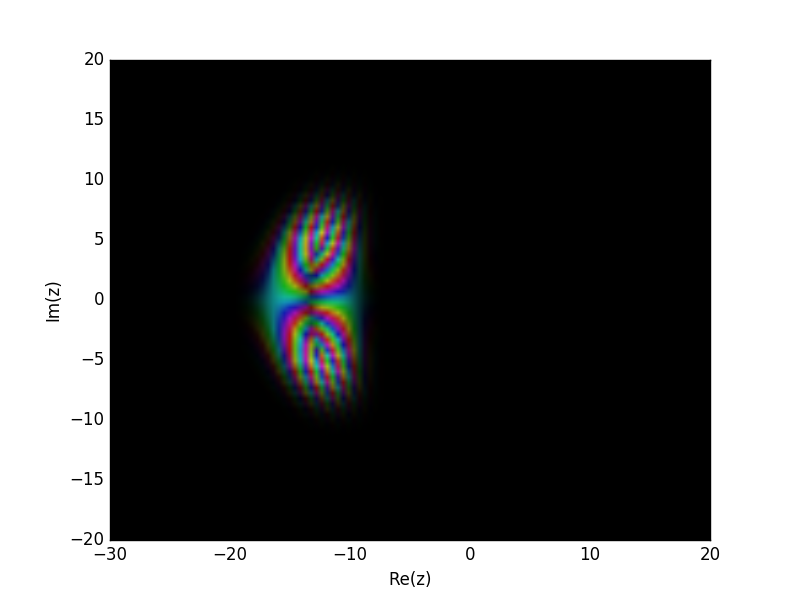
\includegraphics[height=0.8\textheight]{phase_portrait_0.png}
    \end{figure}}

    \only<2>{\begin{figure}[h]
        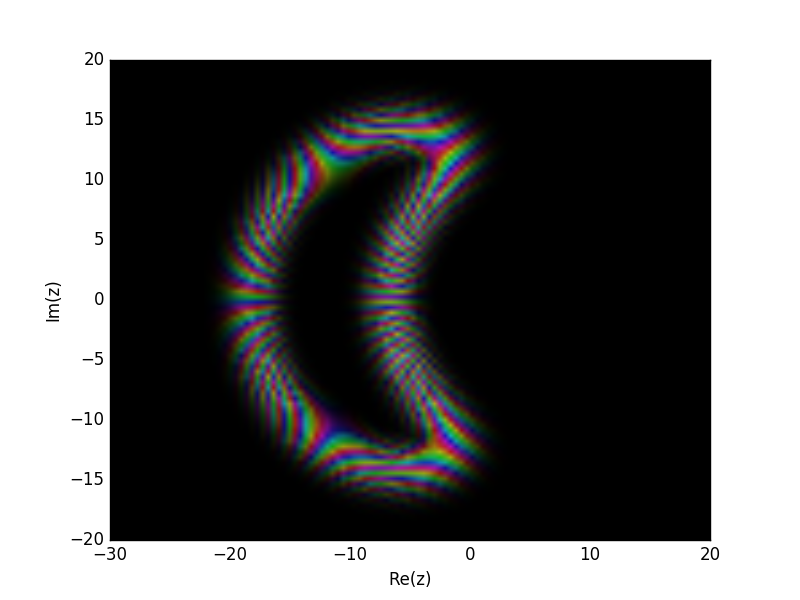
\includegraphics[height=0.8\textheight]{phase_portrait_1.png}
    \end{figure}}

    \only<3>{\begin{figure}[h]
        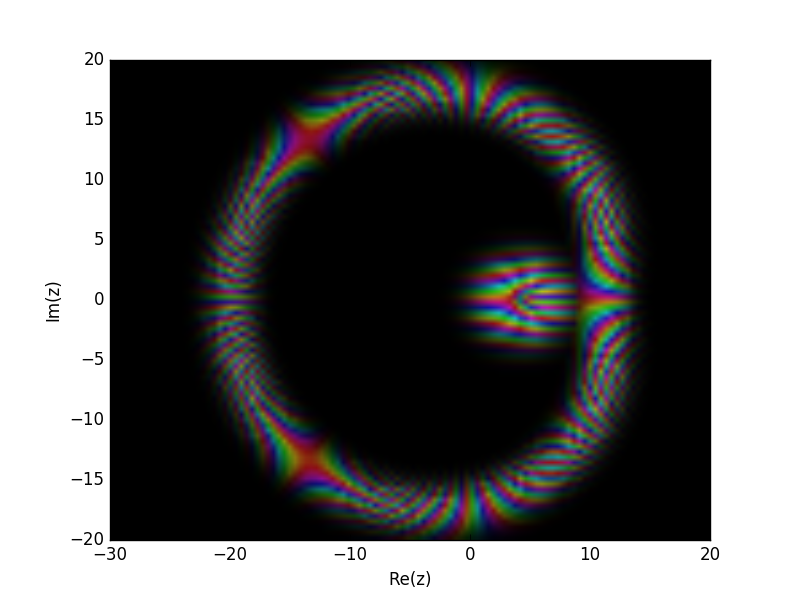
\includegraphics[height=0.8\textheight]{phase_portrait_2.png}
    \end{figure}}
    
\end{frame}

\begin{frame}
    \frametitle{Bistability}
    Bistability means that there exist {\color{red} two stationary points} on the phase diagram. 
    In the presence of dissipation, the oscillator evolves to one of them.

    \begin{block}{''Quantum`` bistability}
    It's necessary to introduce some relaxation to understand bistability in quantum case. With
    relaxation, it is reasonable to expect two peaks in occupation numbers.
    \end{block}
\end{frame}

\begin{frame}
    \frametitle{Oscillator with dissipation}
    A nonlinear oscillator interacting with a bath:    
    \begin{equation*}
        \begin{gathered}
            \hat{H}_{\mathrm{full}} = \hat{H} + \hat{H}_\mathrm{bath} + \hat{H}_\mathrm{int}, \\
            \hat{H}_\mathrm{bath} = \sum \omega_k b_k^\dagger b_k \\
            \hat{H}_\mathrm{int} = \sum \gamma_k a^\dagger b_k + \mathrm{h. c.}
        \end{gathered}
    \end{equation*}
\end{frame}

\begin{frame}
    \frametitle{Oscillator with dissipation}
    In rotating frame,
        
    \begin{multline*}
        \hat{H}_\mathrm{eff} = (\omega_0 - \Omega) a^\dagger a + 
                            \frac{\beta}{2} a^\dagger a^\dagger a a + 
                    E^* a + Ea^\dagger + \\
                    + \sum (\omega_k - \Omega) b_k^\dagger b_k + 
                    \sum \gamma_k a^\dagger b_k + \mathrm{h. c.}
    \end{multline*}
    Now the bath contains oscillators with negative energy!
\end{frame}

\begin{frame}
    \frametitle{Kinetic equation}
    According to the golden Fermi rule,
    \begin{equation*}
        \begin{gathered}
            \frac{dP(m \leftarrow n)}{dt} \propto | \gamma_k \langle \psi_m | \hat{a} | \psi_n \rangle|^2,\\
            \omega_k - \Omega = E_n - E_m
        \end{gathered}
    \end{equation*}
    That allows to write a kinetic equation:
    \begin{equation*}
        \frac{dP_m}{dt} = \sum_n \frac{dP(m \leftarrow n)}{dt} P_n - \frac{dP(n \leftarrow m)}{dt} P_m
    \end{equation*}
    Matrix elements $\langle \psi_m | \hat{a} | \psi_n \rangle$ can be computed numerically, and
    $\gamma(E)$ can be defined phenomenologically as $\propto \theta(E)$ or $\propto E,\, E > 0$.
\end{frame}

\begin{frame}
    \frametitle{Distributions of occupation numbers}
    \begin{equation*}
    \omega_0=1,\, \Omega=1.025,\, \beta=0.001
    \end{equation*}
    \only<1>{
    \begin{columns}
        \begin{column}{0.5\textwidth}
            \centering
            \begin{figure}
                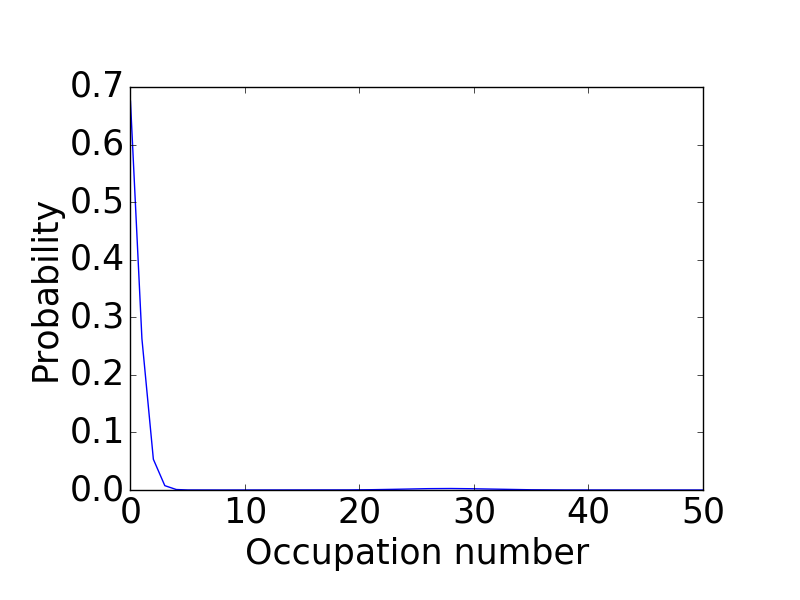
\includegraphics[height=0.45\textheight]{bistability_E015160.png}
                \caption{$E = 0.01516$}
            \end{figure}
        \end{column}
        \begin{column}{0.5\textwidth}
            \begin{figure}
                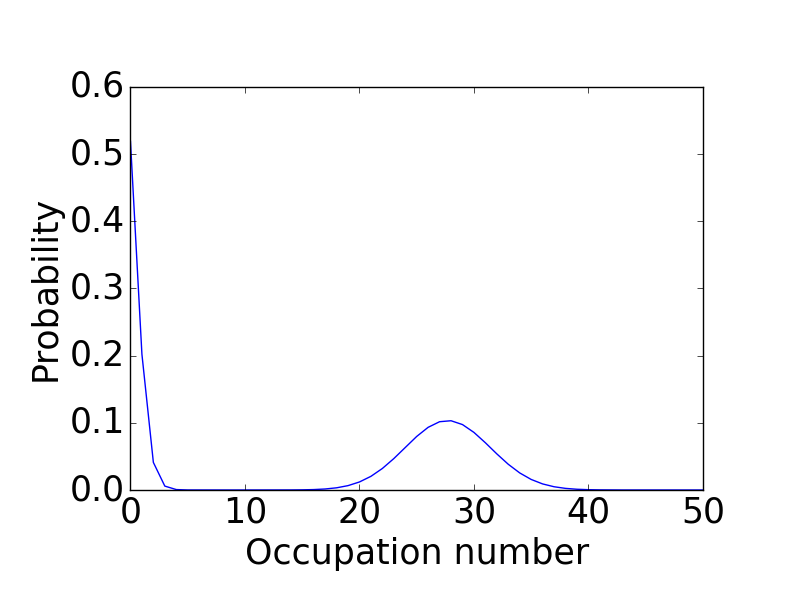
\includegraphics[height=0.45\textheight]{bistability_E015165.png}
                \caption{$E = 0.015165$}
            \end{figure}
        \end{column}
    \end{columns}}

    \only<2>{
    \begin{columns}
        \begin{column}{0.5\textwidth}
            \centering
            \begin{figure}
                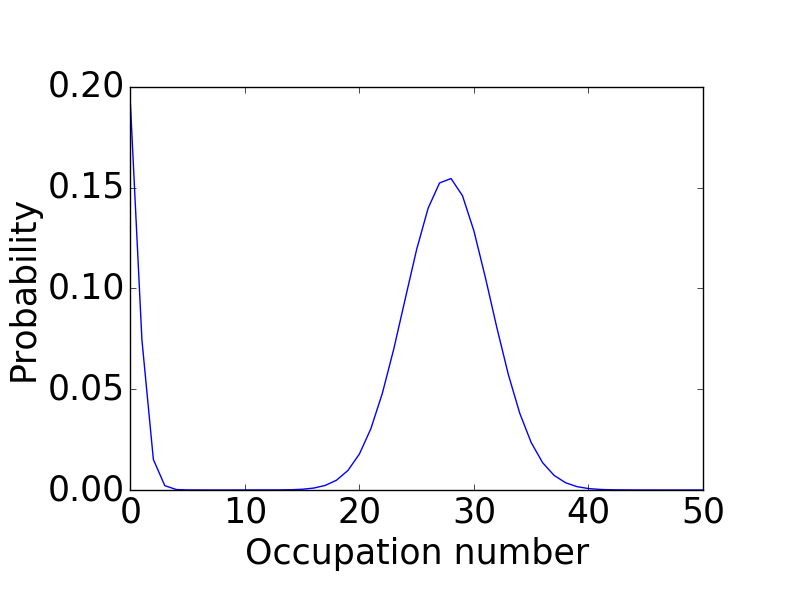
\includegraphics[height=0.45\textheight]{bistability_E015170.png}
                \caption{$E = 0.015170$}
            \end{figure}
        \end{column}
        \begin{column}{0.5\textwidth}
            \begin{figure}
                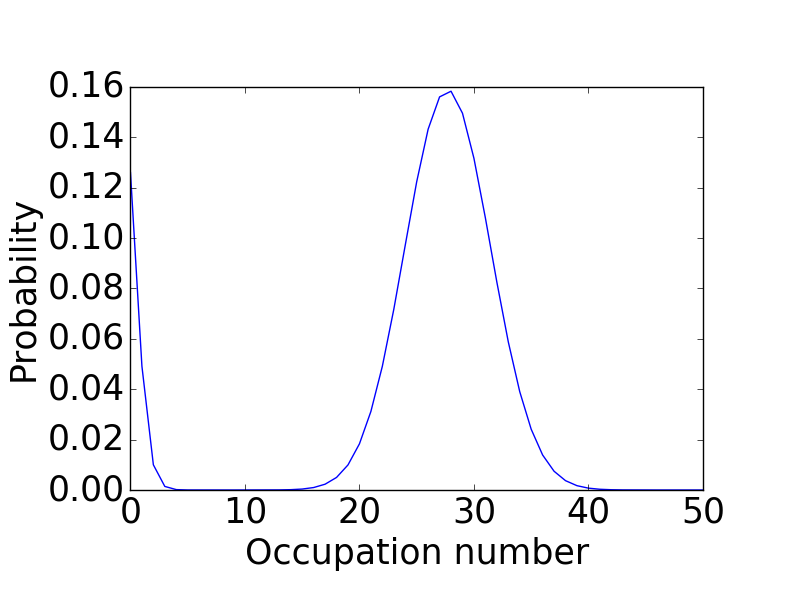
\includegraphics[height=0.45\textheight]{bistability_E015175.png}
                \caption{$E = 0.01575$}
            \end{figure}
        \end{column}
    \end{columns}}
\end{frame}

\end{document}
